\subsection{Root Zonation}

The growing root of \emph{A. thaliana} can be roughly divided into six distinct zones, with the cells in each zone exhibiting qualitatively distinct behaviour. At the tip of the root lies the root cap, a region of cells that are constantly sluffed off to protect the growing root from debris (\cite{kumpf2015}). Above the root cap is a small group of static cells known as the quiescent centre (henceforth QC), which play a crucial role in the regeneration of the root cap and surrounding cells (\cite{matosevich2021}). The models presented in this paper will ignore these two regions and measure position within the root as the distance in $\um$ from the QC. 

\medskip

In the meristematic zone (henceforth MZ), cells experience rapid cell division and slower cell growth. In this region, cells grow from $4.5\um$ to $9\um$ over a period of about $18\h$ (\cite{verbelen2006}) while moving from $0\um$ to $200\um$ above the QC. Above the meristematic zone is the transition zone (henceforth TZ), in which cells grow from $9\um$ to $30\um$ over the course of $10\h$ (\cite{verbelen2006}). Microscopy imaging found the CDC2 protein kinase in epidermal cells in the distal region of the TZ, which suggests that some cells in the TZ have the capacity for division (\cite{verbelen2006}). The TZ spans from approximately $200\um$ to $520\um$ above the QC. Next to the TZ is the elongation zone (henceforth EZ), where cells grow rapidly from $30\um$ to $130\um$ over the course of $4\h$ (\cite{verbelen2006}). After leaving the EZ at approximately $900\um$ above the QC, cells begin differentiation and cease growth. Thus the final and most proximal region of the root is aptly named the differentiation zone (henceforth DZ).

\subsection{CLASP and Microtubules}

Microtubules (henceforth MTs) are tubulin polymers located on the plasma membrane of the cell which guide the deposition of cellulose on the cell wall (\cite{hamant2010}). When the MTs and cellulose microfibrils are deposited orthogonally to the axis of growth, the cell experiences anisotropic growth. If the MTs and cellulose are less organized, then the turgor pressure within the cell faces isotropic resistance which ultimately inhibits growth (\cite{hamant2010}).

\medskip

The CLASP protein plays an essential role in MT patterning through its ability to help MTs cross sharp edges on the cell membrane (\cite{ambrose2011}). This results formation of bundles of MTs along the transverse, radial, and longitudinal edges of the cell (\cite{halat2022}). Bundles along the transverse and radial edges (henceforth TFBs), are of particular interest because they lead to microtubule arrangements that run parallel to the axis of growth.
These TFBs disrupt the formation of circumferential cellulose microfibrils, which ultimately inhibits cell growth (\cite{halat2022}). Cell length modulates the effect of CLASP on MT patterning due to the fact that longer cells have longer longitudinal edges relative to their radial and transverse edges. Therefore, the CLASP protein to localizes towards the longitudinal edges and away from the radial and transverse edges in longer cells, leading to a reduction in TFBs and an increase in growth (\cite{halat2022}). 

\subsection{Brassinosteroid}

Brassinosteroids (BRs) are a class of plant hormones that have shown to promote both longitudinal and radial growth in a spatiotemporal manner (\cite{ackerman-lavert2020}). Extracellular BRs, particularly brassinoslide (henceforth BL), bind to the BR receptor BRI1 and its homologues on the cell membrane (\cite{vukasinovic2021}). This releases the inhibition of the BZR1/BES1 transcription factors by the BIN2 signalling inhibitor (\cite{ackerman-lavert2020}). The effects of BR signalling have been shown to be stronger in the TZ and stronger still in the EZ due to a higher concentration of BR precursors (\cite{vukasinovic2021}). 

\medskip

The BZR1/BES1 transcription factors, which are often used as a proxy for BR signalling, have been shown to inhibit CLASP by binding directly to its promoter and repressing its activity (\cite{ruan2018}). Additionally, CLASP influences the BR signalling network by promoting the recycling of endocytosed BRI1 receptors. Together, these two effects produce a stable postive-negative feedback loop that helps to ensure homeostasis in the root (\cite{ruan2018}).

\subsection{Mutant Roots}

Making small changes to the network of proteins and hormones described in the prior two sections leads to significant changes in root phenotypes. This paper explores the \emph{clasp-1} (henceforth CLASP-1) (\cite{ambrose2007}) and \emph{brinCLASPpro} (henceforth BRIN-CLASP) (\cite{ruan2018}) mutant roots. The CLASP-1 root has a loss-of-function mutation that entirely inhibits the production of CLASP, which ultimately leads to an increase in cell growth through the previously discussed pathway (\cite{halat2022}). However, the rapid cell growth results in fewer cell divisions and thus fewer cells in the CLASP-1 root (\cite{halat2022}), resulting in a lower rate of overall root growth relative to the wild type (\cite{ambrose2007}). 


\medskip

In wild type roots, the transcription of the CLASP protein is inhibited whenthe root is exposed to exogenous BRs (\cite{ruan2018}). However, the BRIN-CLASP root is insensitive to the effects of BR signalling, meaning the application of exogenous BRs does not affect the amount of CLASP in this mutant. It therefore stands to reason that the BRIN-CLASP mutant should have more CLASP than the wild type due to the abscence of this inhibition. It has been shown that an excess of CLASP upregulates the level of BR signalling by promoting the recycling of BRI1 receptors (\cite{ruan2018}), and we speculate that this leads to the increased cell growth observed in BRIN-CLASP mutants relative to the wild type. A plot of cell size in trichoblast cells from the mutants and the wild type is shown in Figure \ref{fig:mutant-sizes}. 

\medskip

\begin{figure}
    \centering
    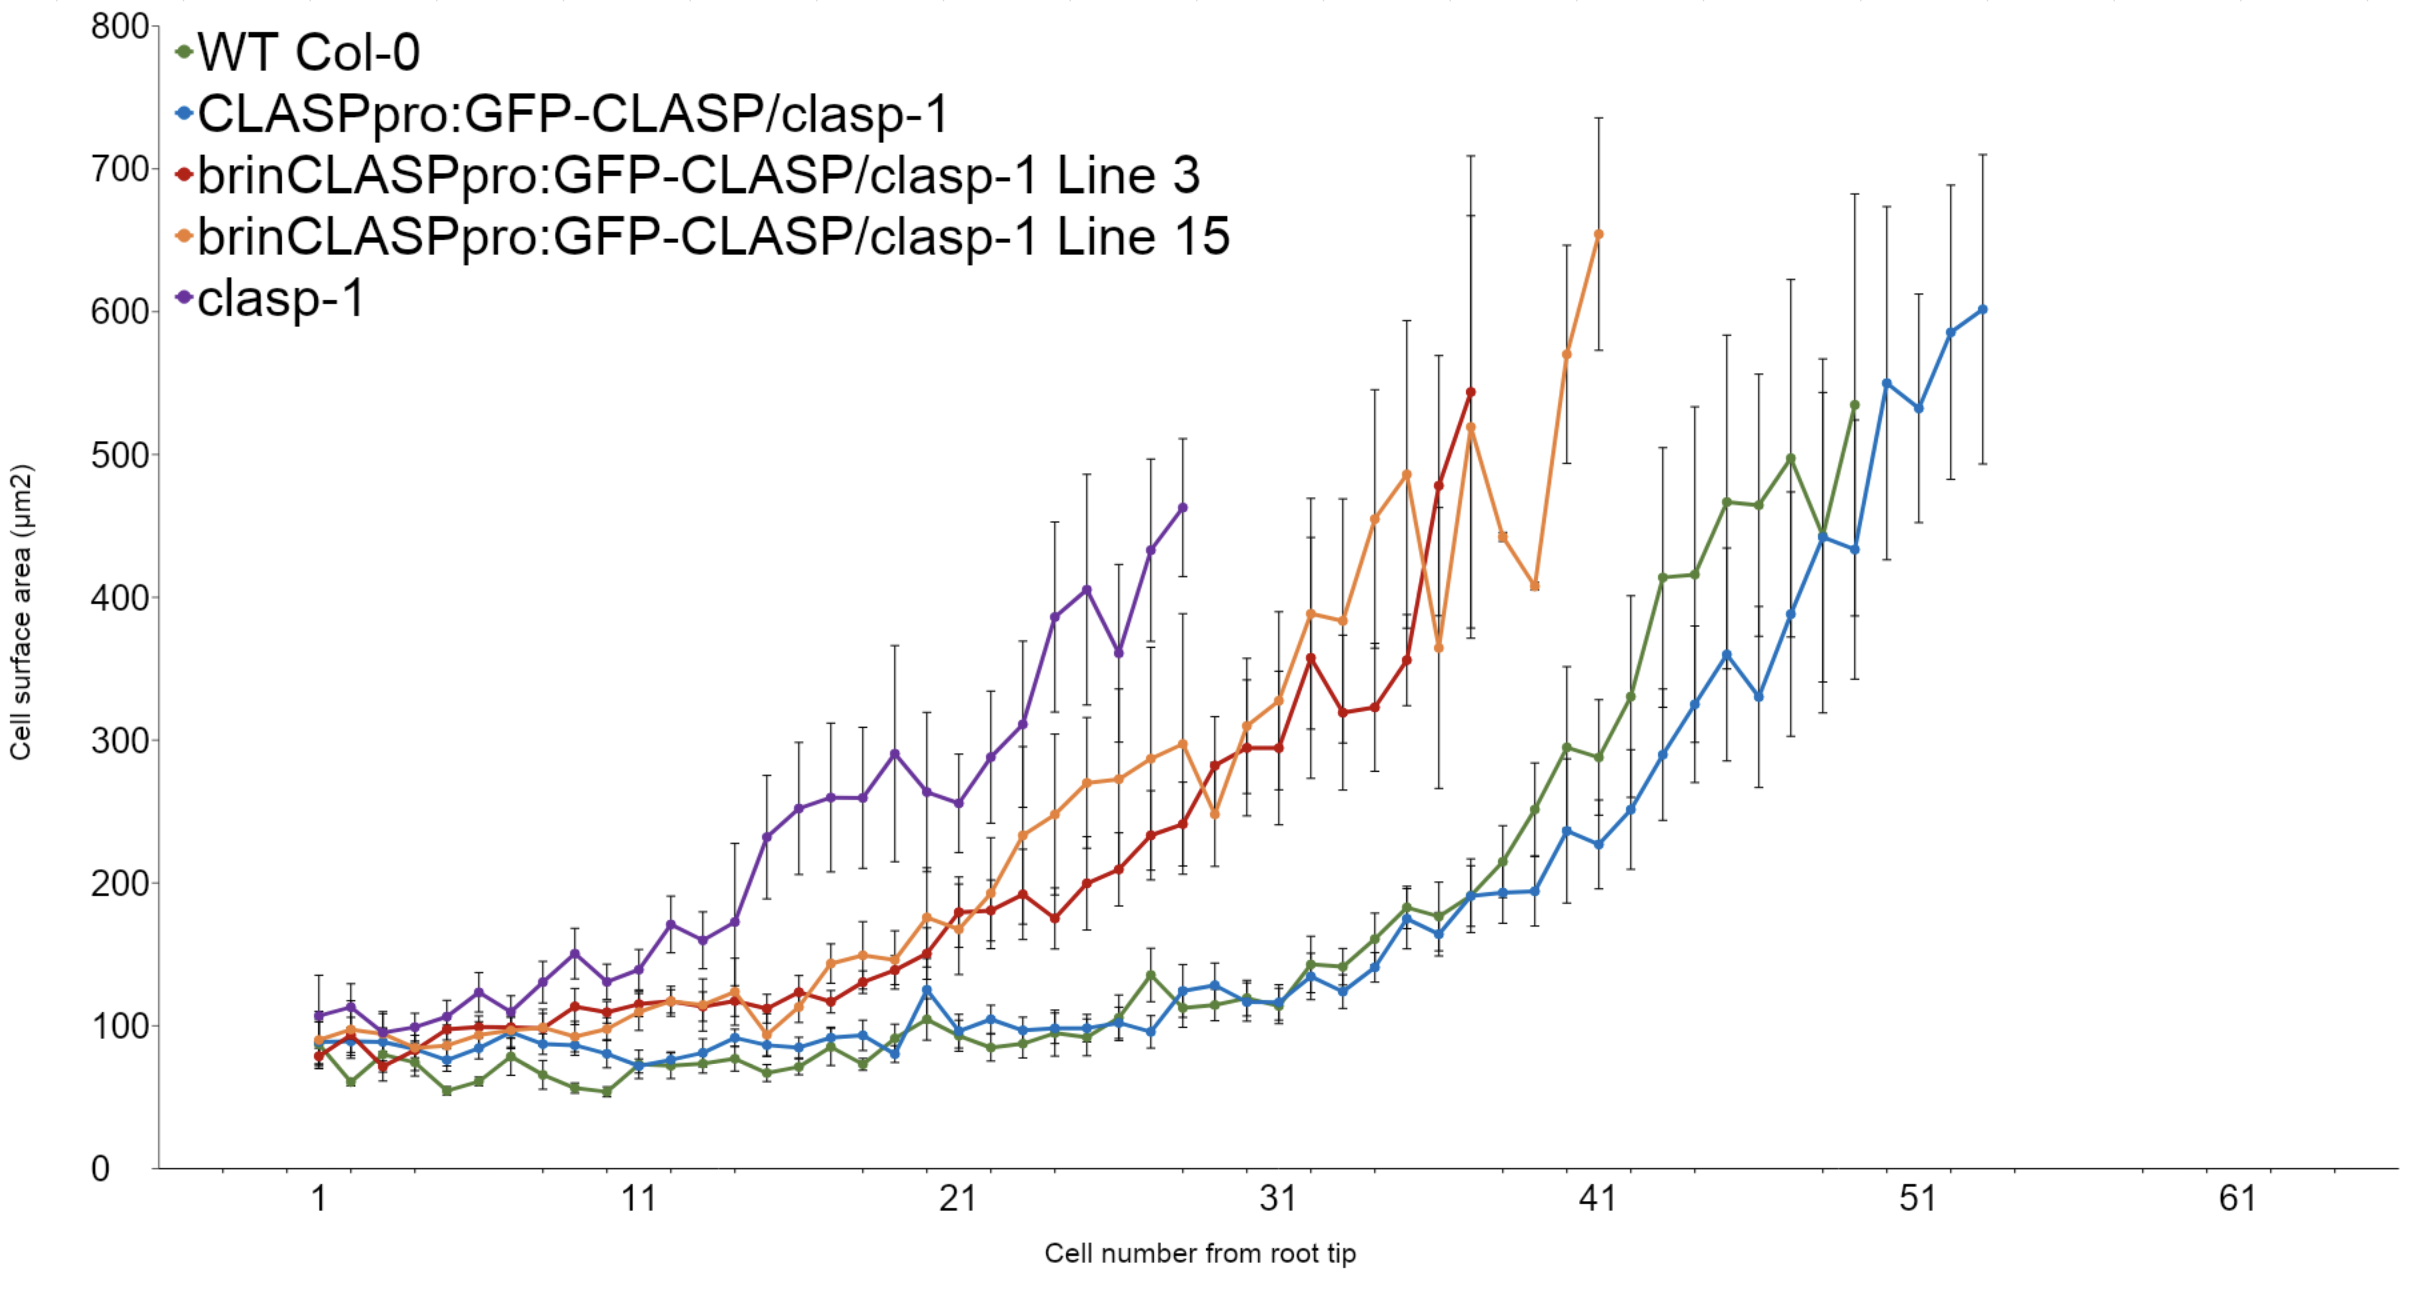
\includegraphics[width=13cm]{img/mutant-cell-sizes.png}
    \caption{Average cell areas plotted against cell number for each of the two mutant roots and the wild type. The GFP-CLASP line drives the expression of a fluorescent fusion protein which fully complements the CLASP-1 mutant (\cite{ambrose2011}). Therefore, the GFP-CLASP/clasp-1 root is phenotypically similar to the wild type. Observe that the CLASP-1 mutant has the largest cells, followed by the BRIN-CLASP mutant, followed by the wild type.}
    \label{fig:mutant-sizes}
\end{figure}







